
%%%%%%%%%%%%%%%%%%%%%%% file typeinst.tex %%%%%%%%%%%%%%%%%%%%%%%%%
%
% This is the LaTeX source for the instructions to authors using
% the LaTeX document class 'llncs.cls' for contributions to
% the Lecture Notes in Computer Sciences series.
% http://www.springer.com/lncs       Springer Heidelberg 2006/05/04
%
% It may be used as a template for your own input - copy it
% to a new file with a new name and use it as the basis
% for your article.
%
% NB: the document class 'llncs' has its own and detailed documentation, see
% ftp://ftp.springer.de/data/pubftp/pub/tex/latex/llncs/latex2e/llncsdoc.pdf
%
%%%%%%%%%%%%%%%%%%%%%%%%%%%%%%%%%%%%%%%%%%%%%%%%%%%%%%%%%%%%%%%%%%%


\documentclass[runningheads,a4paper]{llncs}

\usepackage{amssymb}
\setcounter{tocdepth}{3}
\usepackage{graphicx}
%===========moi them vao =====================
%\usepackage{graphicx}
\graphicspath{{figures/}}
%===========moi them vao =====================
\usepackage{url}

\usepackage[noend]{algorithmic}
\usepackage[lined,ruled,commentsnumbered]{algorithm2e}


\urldef{\mailsa}\path|{tbnguyen, olivetti, avesani}@fbk.eu|
\newcommand{\keywords}[1]{\par\addvspace\baselineskip
\noindent\keywordname\enspace\ignorespaces#1}

\begin{document}

\mainmatter  % start of an individual contribution

% first the title is needed
\title{Multiple scales for visulalization large data}

% a short form should be given in case it is too long for the running head
\titlerunning{Multiple scales for visulalization large data}

% the name(s) of the author(s) follow(s) next
%
% NB: Chinese authors should write their first names(s) in front of
% their surnames. This ensures that the names appear correctly in
% the running heads and the author index.
%

\author{Thien Bao Nguyen%
%\thanks{Please note that the LNCS Editorial assumes that all authors have used the western naming convention, with given names preceding surnames. This determines the structure of the names in the running heads and the author index.}%
\and Emanuele Olivetti\and Paolo Avesani}
%
\authorrunning{Multiple scales for visulalization large data}
% (feature abused for this document to repeat the title also on left hand pages)

% the affiliations are given next; don't give your e-mail address
% unless you accept that it will be published
\institute{NeuroInformatics Laboratory (NILab),\\
     Bruno Kessler Foundation, Trento, Italy\\
	Centre for Mind and Brain Sciences (CIMeC),\\
    University of Trento, Italy \\
%Springer-Verlag, Computer Science Editorial,\\
%Tiergartenstr. 17, 69121 Heidelberg, Germany\\
\mailsa \\
%\mailsb\\
%\mailsc\\
%\url{http://www.springer.com/lncs}
}

%
% NB: a more complex sample for affiliations and the mapping to the
% corresponding authors can be found in the file "llncs.dem"
% (search for the string "\mainmatter" where a contribution starts).
% "llncs.dem" accompanies the document class "llncs.cls".
%

\toctitle{Multiple scales for visulalization large data}
\tocauthor{Authors' Instructions}
\maketitle

\begin{abstract}
  We developed a novel interactive system for human brain tractography
  segmentation to assist neuroanatomists in identifying white matter
  anatomical structures of interest from diffusion magnetic resonance
  imaging data (dMRI). The difficulty in segmenting and navigating
  tractographies lies in the very large number of \emph{streamlines},
  in the order of hundreds of thousands, that modern MR techniques
  provide. The novelty of our system resides in presenting a clustered
  version of the tractography to the user which interactively selects
  the clusters of interest to narrow down the initial tractography to
  a subset containing the anatomical structure. The set of streamlines
  of the selected clusters are then re-clustered in smaller clusters
  so that the user can refine the previous selection and then
  re-cluster again at a finer scale. This process is iterated until
  the union of the remaining clusters faithfully represent the desired
  structure. The proposed system adopts a solution to solve the
  computational issue of clustering a large number of streamlines
  under the strict time constraints requested by the interactive
  use. The solution consists in projecting the streamlines into a
  Euclidean space and then in adopting a state-of-the art scalable
  implementation of the $k$-means algorithm. We tested the proposed
  system on tractographies from amyotrophic lateral sclerosis (ALS)
  patients and healthy subjects to study the systematic differences
  within the corticospinal tract.
\end{abstract}

%%% Local Variables: 
%%% mode: latex
%%% TeX-master: "olivetti_boi"
%%% End: 


\keywords{ Visualization, Hierarchical Clustering, Machine Learning, Large Data, Tract Segmentation, dMRI Data}

\section{Introduction}
\label{sec:introduction}
%the need of visualization data
To support human in analyzing and exploring large data, it is an important task to graphically present the data~\cite{yang2003interactive}. Users, in one side, have a requirements of looking at complex and intricate data to find out some facts or trends that are not esy to find. On the other side, they want to explore data in details to examine each data points. In fact, the overall premise is that users have a deeper understanding about their data when they interact with the presented information and view it at different levels of abstraction~\cite{roberts2007state}. During the last two decades, many interactive visualization techniques and system have been emerged~\cite{yang2003interactive,stroe2000scalable,fua2000structure}.
As large data sets become more and more common, with the oder over $1K$, it has been clear that most of the current visualization approaches lose their effectiness due to they have no ability to visualize and manage the large number of data points simultaneously. In this scenerio, clustering is considered a suitable method for understanding and to exploring large data~\cite{berkhin2006survey,bisson2012improving}. 
However, clustering usually results in one partition of the data, and this leads to the drawback because the validation process is not straightforward due to the lack of grouth truth data~\cite{candillier2006casade}. One solution for this is hierarchical clustering~\cite{johnson1967hierarchical}, which organizes data in an intutive and interpretable way, namely dendrogram, not only one partion as the traditional clustering methods.
%In such tructure, all the degree of generality are present 
This character allows users to explore in a simple way the clusters and the relationships between instances, leading to many applications for visulization~\cite{heard2009novel,landesberger2011visual,mahe2009graph}.
%what is the limitation of current visualization method to large data
Nevertheless, when dealing practically with a large size dendrogram, it becomes difficult since the number of leaves grows exponentially with the depth of the tree and makes users lose the overview of the whole dataset. To deal with this prolbem, many sugguestion have been approached~\cite{bisson2012improving,landesberger2011visual,furnas2006fisheye}. However, these methods are either display at one time only a subpart of the structure~\cite{landesberger2011visual,furnas2006fisheye}, or display whole dendrogram but rely on other clustering technique~\cite{bisson2012improving}.

%Contents of the paper
In this work, we propose a framework of offering a complete and interactive visualization of the large data. Our method allow users to apply his or her perceptual abilities to make sense of data. 
%We describe the algorithmic solutions we adopted in order to build the interactive visualization large data.  
The core of the problem is to obtain the multiple scales for representation large data in order to comply with the requirements of human interactive visualization. The proposed solution combines three steps. First, the dendrogram would be created by running the hierarchical clustering. Second, the \emph{goodness} function is used as a measurement to select the most relevant scales for representing the dendrogram. Lastly, we also evaluate the multipe scales based on a application deriven criteria, called \emph{split factor}. 

% tractography segmentation tool. The core of the problem is to obtain fast clustering of a large number of streamlines in order to comply with the requirements of human interaction. The proposed solution combines two state-of-the-art elements: first a recently proposed Euclidean embedding algorithm for streamlines, i.e. the dissimilarity representation with the scalable \emph{subset farthest first} (SFF) prototype selection policy~\cite{olivetti2012approximation}. This embedding provides fast and accurate vectorial representation of streamlines, needed by most of the clustering algorithms. Second, a recently proposed improvement of the $k$-means clustering algorithm called \emph{mini-batch} $k$-means~\cite{sculley2010web} (MBKM). This algorithm drastically reduces the convergence time to the actual clusters in case of large and very-large sets of objects. We also tested a further potential improvement, i.e. a recently proposed initialisation algorithm for the $k$-means family, called $k-means++$~\cite{arthur2007kmeans}. But we excluded it from the final system due to poor performance as illustrated in Section~\ref{sec:experiments}.

% Structure of the paper
The paper is organized as follows. Section~\ref{sec:methods} introduces the
algorithmic elements of the proposed method including hierarchical clustering, multiple scales choosing and quantitatively evaluating the goodness of the representation. In section~\ref{sec:experiments}, we describe details of the actual use of the proposed solution in the context of the tractgoraphy segmentation, provide figures to evaluate the viability of the proposed solution. We conclude with a summary of our contribution and open areas for future work in the last section~\ref{sec:conclusion}.
%  and are formally described
%We quantitatively describe the segmentation process and provide figures to evaluate the viability of the proposed solution. In Section~\ref{sec:discussion} we discuss the results and we show that the proposed solution is effective. We conclude by mentioning the future steps for the development of our software, called \emph{spaghetti}, and the open computational challenges that needs to be solved.



\section{Methods}
\label{sec:methods}
In the following we describe the elements that we evaluated in order
to build the proposed method. After introducing the notation we
formally describe the dissimilarity representation, i.e. a Euclidean
embedding for streamlines, and then we present the mini-batch
$k$-means algorithm. We conclude by reporting how we efficiently
compute the medoids of the clusters from the centroids.

\subsection{Notation}
\label{sec:notation}
Let $X \in \mathcal{X}$ be a streamline, i.e. a sequence of points in
$3$D space $X = \left((\mathbf{x}_1),\ldots,(\mathbf{x}_n)\right)$,
$\mathbf{x} = (x,y,z) \in \mathbb{R}^3$. Notice that in general $n$ is
different from one streamline to another, which means that streamlines
are heterogeneous objects that cannot be directly represented as
vectors of the same vector space. Let $T = \{X_1,\ldots,X_M\}$ be a
brain tractography, for which $M \approx 3 \times 10^5$ usually. Let
$d:\mathcal{X} \times \mathcal{X} \mapsto \mathbb{R}^+$ be a distance
function between streamlines. A common distance between streamlines is
the symmetric minimum average distance
(see~\cite{zhang2008identifying}) defined as $d(X_a,X_b) =
\frac{1}{2}(\delta(X_a,X_b) + \delta(X_b,X_a))$ where
\begin{equation}
  \label{eq:mam_distance}
  \delta(X_a,X_b) = \frac{1}{|X_a|} \sum_{\mathbf{x}_i \in X_a}
    \min_{\mathbf{y} \in X_b} ||\mathbf{x}_i - \mathbf{y}||_2.
\end{equation}



\subsection{The Dissimilarity Representation}
\label{sec:dissimilarity}
The \emph{dissimilarity representation}~\cite{pekalska2002generalized}
is a lossy Euclidean embedding algorithm that maps general objects
into vectors of a common vectorial space $\mathbb{R}^p$. In our case
these objects are the streamlines, as it was previously proposed
in~\cite{olivetti2012approximation}. The dissimilarity representation
is a function $\phi_{\Pi}^d(X):\mathcal{X} \mapsto \mathbb{R}^p$ s.t.
\begin{equation}
  \phi_{\Pi}^d(X) = [d(X,\tilde{X}_1) ,\ldots, d(X,\tilde{X}_p)]
\label{eq:dissimilarity_representation}
\end{equation}
where $d$ is a given distance function between streamlines, and $\Pi =
\{\tilde{X}_1, \ldots, \tilde{X}_p\} \subset \mathcal{X}$ is a given
set of $p$ streamlines called \emph{prototypes} or
\emph{landmarks}. The quality of the Euclidean embedding is strongly
dependent on the choice of $d$ and on the selection of the prototypes
(see~\cite{pekalska2006prototype,olivetti2012approximation}). In this
work we adopt the distance of Equation~\ref{eq:mam_distance}, as
suggested in~\cite{olivetti2012approximation,zhang2008identifying}.

An efficient procedure to select effective prototypes in the case of
tractography data was presented in~\cite{olivetti2012approximation}:
the \emph{subset farthest first} (SFF) algorithm. This procedure is a
scalable approximation of the well known farthest first traversal
(FFT) algorithm.
% which is a standard greedy solution to the well known $k$
% centre problem. This problem, put in our context, entails selecting a
% set $\Pi$ of $p$ streamlines~\footnote{Note that here we use $p$ to
%   denote the size of $\Pi$ instead of the $k$ of the ``$k$ centre
%   problem''. This is to avoid confusion with the notation we adopt in
%   this paper.} such that the sum of the distances of each streamline
% of the tractography to closest streamline in $\Pi$ is minimised.
% % Intuitively the streamlines in $\Pi$ are designed to be a
% % \emph{representative} sample of the whole tractography.
The FFT algorithm selects one streamline at random from the
tractography as the first prototype $\tilde{X}_1$ and then iteratively
adds a new prototype as the streamline maximising the distance to the
already selected prototypes. The SFF algorithms is a stochastic
scalable version of FFT, which subsamples $m = \lceil c p \log p
\rceil$ streamlines from the whole tractography, and then applies FFT
to the subsample. For the case of tractography data, when $c>=3$ the
SFF algorithm is comparable to the FFT algorithm with high
probability, following the proof in~\cite{turnbull2005fast} and the
empirical results in~\cite{olivetti2012approximation}.


\subsection{Mini-Batch $k$-means}
\label{sec:mbkm}
The $k$-means clustering problem is a cornerstone of the clustering
literature. Given $k$, the number of clusters, the problem is to find
$k$ cluster centres $C = \{\mathbf{c}_1,\ldots,\mathbf{c}_k\}$,
$\mathbf{c} \in \mathbb{R}^p$, and to assign each element of the
vectorial dataset $\Phi(T) = \{\phi(X_1),\ldots,\phi(X_M)\} \subset
\mathbb{R}^p$ to the closest cluster\footnote{From now on, we denote
  $\phi_{\Pi}^d(X)$ as $\phi(X)$ to simplify the notation without
  introducing ambiguity.}. The $k$-means problem is then to compute
centres $C$ such as to minimise the loss function
\begin{equation}
  \label{eq:kmeans_loss}
  \min \sum_{\phi(X) \in \Phi(T)} D(\phi(X),C)^2
\end{equation}
Where $D(\phi(X),C) = \min_{\mathbf{c} \in C}||\phi(X) -
\mathbf{c}||_2$ is the distance between $\phi(X)$ and the closest
centre. The exact solution of the $k$-means problem is $NP$-hard and
the computational complexity of the standard algorithm, the Lloyd's
algorithm~\footnote{\url{http://en.wikipedia.org/wiki/K-means_clustering#Standard_algorithm}},
has been proved to be $O(M^{34})$ in the general
case~\cite{arthur2009kmeans}, even though much less in practical
applications. Nevertheless the standard algorithm impractical when
clustering a tractography data in an interactive setting, as we show
in Section~\ref{sec:experiments}.

The \emph{mini-batch $k$-means} (MBKM) algorithm~\cite{sculley2010web}
is a recently proposed modification of the standard algorithm that is
able to reduce the computational costs by orders of magnitude. The
intuitive idea is to use a stochastic gradient descent approach to
find the centres $C$ starting from a random initialisation. This idea
was introduced in~\cite{bottou1995convergence} where the points of the
dataset were given one at a time in an online fashion.

Instead of updating the centers with one streamline at a time, the
MBKM algorithm proposes to use multiple random subsets of the dataset,
i.e. the \emph{mini batches}, to update the cluster centres and to
estimate the per-centre learning rates. As soon as the objective
function in Equation~\ref{eq:kmeans_loss} converges the process
stops. The pseudocode algorithm of MBKM is shown
in~\cite{sculley2010web} and we do not report it here for lack of
space.

The computational complexity of the MBKM algorithm is not known in the
general case but empirical results in~\cite{sculley2010web} show a
reduction of two orders of magnitude in computation time with respect
to the standard $k$-means. We present analogous results on
tractography data in Section~\ref{sec:experiments}.



\subsection{From Centroids to Medoids}
\label{sec:trees}
In order to visually present the clusters of streamlines to the user
one representative streamline of each cluster needs to be selected. In
the general case the dissimilarity representation is not invertible,
i.e. given a vector $\mathbf{c} \in \mathbb{R}^p$ it is not possible
to construct the streamline $X_{\mathbf{c}}$ such that $\mathbf{c} =
\phi{X}$. This means that the centroids $C$ obtained with the
$k$-means or the MBKM cannot be shown to the user as streamlines. For
this reason we decided to display the \emph{medoid} of each cluster,
i.e. the streamline of the tractography closest to each centroid
$\mathbf{c}$. The exhaustive search of the medoids requires the
computation of $kM$ distances, which is too slow for interactive
use. For this reason we adopted a data structure for efficient
computation of the nearest neighbour in high-dimensional spaces: the
\emph{Ball Tree}. We refer the reader to~\cite{omohundro1989balltree}
for additional details. We present empirical results of the time
required for the computation of the medoids in
Section~\ref{sec:experiments}.

%%% Local Variables: 
%%% mode: latex
%%% TeX-master: "olivetti_boi"
%%% End: 



%\section{Evaluation}
\label{sec:evaluation}
Before proceeding with our main experiments, we first clarify some notation and introduce the hierarchical model the we will analyze. 
\subsection{Hierarchical clustering}
\label{subsec:hierarchical}
Given a set of input patterns denoted as $\mathcal{X} = \{\mathsf{x_1}, \ldots, \mathsf{x_j}, \ldots, \mathsf{x_N}\}$ where $\mathsf{x_j} = (x_{j1},x_{j2}, \ldots,x_{jd})^T \in \mathfrak{R}^d$ and each measure $x_{ji}$ is said to be a feature (attribute, dimension, or variable). Hierarchical clustering~\cite{johnson1967hierarchical} produces a structure of clusters of $\mathcal{X}$ that is more informative than the unstructured set of clusters returned by flat clustering. 
This characteristic meets the requirement of creating multiple scales of one original dataset $\mathcal{X}=\{x_1, \ldots, x_n\}$ 
%$\mathbb{P}$ of $\mathcal{T}$ 
%the immediately responding to the changing level of abstraction of user 
without re-running the clustering algorithm again. Another advantage is that hierarchical clustering does not require to pre-specify the number of clusters. It builds nested clusters by merging them successively, and this hierarchy of clusters represented as a tree (or dendrogram). The root of the tree is the unique cluster that gathers all the samples, the leaves being the clusters with only one sample. In another way, hierarchical clustering algorithm % (http://scikit-learn.org/stable/modules/clustering.html) 
can clusters data firstly on $n$ centers and consequently until only one center. This main character leads to the capability of visualizing $\mathcal{X}$ in many levels of abstraction, and the users can browse the value of level from $1$ to $N$, to see the clusters immediately.
%We refer \mathbb{H} as the whole hierarchical tree or dendogram of $\mathcal{X}$.

\textbf{Definition 1} A \textit{\textbf{hierarchical tree}} $\mathcal{H}$ on objects $\mathcal{X}=\{\mathsf{x_1}, \ldots, \mathsf{x_j}, \ldots, \mathsf{x_N}\}$ is a collection of $Q$ partitions on $\mathcal{X}$: $\mathcal{H}=\{\mathsf{P}_0,\ldots,\mathsf{P}_Q\}$, with $Q \leq N$, such that $\mathsf{P}_0=S$ and $C_{i} \in P_{m}, C_{j} \in P_{l}, m > l$ imply $C_{i} \subseteq C_{j}$ or $C_{i} \cap C_{j} = \emptyset$, for all $i,j \neq i, m, l = 1, \ldots, Q$.

Every hierarchical tree $\mathcal{H}$ has a branch factor parameter $\gamma$ that quantifies how balanced the clusters are at any split.
Formally, $\gamma \geq max_{intras{C_1, \ldots,C_k}} \frac{max_i |C_i|}{min_i |C_i|}$
 where each intra is a non-leaf cluster, partitioned into clusters ${C_1, \ldots, C_k}$. $\gamma$ upper bounds the ratio between the largest and smallest clusters sizes across all intras in cluster $C$. This branch factor has been used in numerous analyses of clustering algorithms~\cite{eriksson2011active,balakrishnan2011noise}, and it is common to assume that the clustering is not too unbalanced.

Hierarchical clustering algorithms are either top-down or bottom-up. Bottom-up algorithms treat each streamline as a singleton cluster at the outset and then successively merge (or agglomerate) pairs of clusters until all clusters have been merged into a single cluster that contains all tracts. Bottom-up hierarchical clustering is therefore called Hierarchical Agglomerative Clustering (HAC). Top-down clustering requires a method for splitting a cluster. It proceeds by splitting clusters recursively until individual streamlines are reached \cite{johnson1967hierarchical}.
The basic process of HAC clustering~\cite{johnson1967hierarchical} is this:
\begin{enumerate}
	\item Assign each object to one cluster. We now have $N$ clusters, each containing just one streamline.
	%Let the distances (similarities) between the clusters the same as the distances (similarities) between the items they contain.
	\item Find the closest (most similar) pair of clusters and merge them into a single cluster.
	\item Compute distances (similarities) between the new cluster and each of the old clusters.
	\item Repeat steps $2$ and $3$ until all streamlines are clustered into a single cluster of size $n$.
\end{enumerate}
Step $3$ can be done in different ways, which distinguishes single-linkage, complete-linkage and average-linkage.
In \emph{single-linkage} clustering (also called the connectedness or minimum method), the distance between a pair of clusters $A$ and $B$ is the shortest distance from any streamline of one cluster to any streamline of the other cluster. 
%If the data consist of similarities, we consider the similarity between one cluster and another cluster to be equal to the greatest similarity from any member of one cluster to any member of the other cluster.
%${d}_sg(A,B) = \min_{i=1,\ldots,n_{s_A}} d({x}_i^A, s_B)$
\begin{equation}
\label{eq:distance_single_linkage}
d(A, B) = \min_{\mathsf{x}_A \in {A},\mathsf{x}_B \in {B}} d(\mathsf{x}_A,\mathsf{x}_B)
\end{equation}
where $d(\mathsf{x}_A,\mathsf{x}_B)$ is the distance between two objects
In \emph{complete-linkage} clustering (also called the diameter or maximum method), we consider the distance between cluster $A$ and cluster $B$ to be equal to the greatest distance from any member of one cluster to any member of the other cluster.
\begin{equation}
\label{eq:distance_complete_linkage}
d(A, B) = \max_{\mathsf{x}_A \in {A},\mathsf{x}_B \in {B}} d(\mathsf{x}_A,\mathsf{x}_B)
\end{equation}
In \emph{average-linkage} clustering, the distance between two clusters $A$ and $B$ is defined as the average distance from any streamline of cluster $A$ to any streamline of cluster $B$.
\begin{equation}
\label{eq:distance_average_linkage}
d(A, B) = avg_{\mathsf{x}_A \in {A},\mathsf{x}_B \in {B}} d(\mathsf{x}_A,\mathsf{x}_B)
\end{equation}

\subsection{Multiple scale for visualization}
\label{sec:multiscale}
The hierarchical tree $\mathcal{H}$ structures and presents dataset $\mathcal{X}$ at different levels of abstraction. A non-leaf cluster is composed of all its child clusters, while a leaf cluster contains only a single data item. The collection of all leaf-clusters presents exactly every data items $\mathsf{x}_i$ of $\mathcal{X}$, while the root is a cluster containing whole dataset $\mathcal{X}$ as one single node of the tree.

\textbf{Definition 2:} Each cluster $C_i$ (node) of the tree $\mathcal{H}$, let $s_i$ be the \textbf{\textit{level of detail}} of that cluster. This measure $s_i$ satisfies the following criteria: if $C_i$ is an ancestor of $C_j$, then $s_i \geq s_j$. 

There are many properties of a cluster which can be used to measure $s_i$. Among of them, two common use are the radius of a cluster (maximum distance between all the pair sample belonging to that cluster $r_i = max_{\forall \mathsf{x}_a, \mathsf{x}_b
 \in C_i, \mathsf{x}_a \neq \mathsf{x}_b} \{d(\mathsf{x}_a,\mathsf{x}_b)\}$); and the hierarchical level of $C_i$ in the tree $\mathcal{H}$ 

\textbf{Definition 3:} The \textbf{\textit{range of scale}} of a hierarchical tree $\mathcal{H}$ is $[s_{min},s_{max}]$, where $s_{min} = min_{\forall C_i \in \mathcal{H}}\{s_i\}$, and $s_{max} = max_{\forall C_i \in \mathcal{H}}\{s_i\}$

Depending on which property is used to measure the level of detail $s_i$, the value of  $s_{max}$ and  $s_{min}$ would be different. In the case of using the hierarchical level, let $h$ be the heigh of the tree $\mathcal{H}$, then the level of detail of cluster $C_i$: $s_i = \frac{height(C_i)}{h}$, where $heigh(C_i)$ is the heigh of the cluster $C_i$. The scale range is $[0,1]$, where $s_{min} = 0$ corresponds to the leaf with zero heigh, and $s_{max} = 1$ is at the root of the tree $\mathcal{H}$. But in the case cluster radius, there is no guarantee that $s_{min} = 0$ and $s_{max} = 1$.

\textbf{Definition 4:} \textbf{\textit{A cut $\mathfrak{L}(w)$}} of a hierarchical tree $\mathcal{H}$ at a given scale $w \in [s_{min},s_{max}] $  is $\mathfrak{L}(w) = \{C_i | (s_i \leq w  \wedge s_{parent(C_i)} > w)\}$, where $parent(C_i)$ is the direct parent of cluster $C_i$

Intuitively, the cut at $s_{min}$, $\mathfrak{L}(s_{max})$ is the set of all leaf clusters, while the $\mathfrak{L}(s_{max})$ is a single cluster representing the whole dataset $\mathcal{X}$. $\mathfrak{L}(w)$ is a partion of $\mathcal{X}$, denoting a subset of the tree $\mathcal{H}$. $\mathfrak{L}(w)$ change smoothly with the variance of the scale parameter $w$, which serves as the abstraction level of the dataset $\mathcal{X}$. It could be imagined that $\mathfrak{L}(w)$ is a cut across a vertically oriented hierarchical tree $\mathcal{H}$ that satisfies criteria: $\mathfrak{L}(w)$ intersecs each path of the tree $\mathcal{H}$, from the root to the leaf, only exactly at one point. The cutting point would depend on the value of parameter $w$. It should close to the root of the tree $\mathcal{H}$ when $w$ is high, and reversely. Beside, the cut can be horizontal or unhorizontal (like zigzag) as long as for each path from the root to the leaf of the tree $\mathcal{H}$, there is only one crossing with $\mathfrak{L}(w)$. It is an open approach for cutting the tree comparing with the traditional one which only accepts the horizontal cut. 

To visualize the dataset $\mathcal{X}$
Scale s = [0,1], where 0 is the whole leaves (streamlines) and 1 is the only one root. Scale s can be defined based on the height of tree h: 0/h, 1/h, ..., (h-1)/h, h/h; or the maximum distance of each node of the tree \cite{yang2003interactive}
How to choose the best scales to cut at, is driven from the paper pons2011postprocessing
Evaluate the cut:
+ At each cutting scale alpha, the result is a partition $P_alpha$ of tractography
+ Measure the quality of a partition P:
- Silhouette Coefficient score: measure of how tightly grouped all the data in the cluster are. The score is bounded between -1 for incorrect clustering and +1 for highly dense clustering. Scores around zero indicate overlapping clusters. The score is higher when clusters are dense and well separated, which relates to a standard concept of a cluster. code [6], paper rousseeuw1987silhouette and web [7]
- Median partition: a good partition is the one which are most similar to all other partitions vega2011segmentation
% HKM (hierarchical k-means objective) & HRC (hierarchical ratio cut): kauchak03iterative

+ Define the target criteria of cutting

- Based on the real fact that user of spagheti usually chose $~15 (k_1)$ clusters which present on the screen is about $~50 (k_2)$representatives (prni2013-boi), we propose a method to evaluate the good cut like that:

+ start from scale $l$, in current partition $P(l)$, draw $S=\{s_1,s_2,..,s_{k_1}\}$ of size $k_1$ uniformly at random

+ calculate branch factor at scale $l$: $b(l) = card(P'(l+1))$, where $P'(l+1) = \{C_i, C_i \in P(l+1), \wedge C_i \in any s_j, with all j =1,..k1\}$

+ set current partition be $P'(l+1)$

+ recursively applying this procedure until we meet the last scale

+ the cut scales are good when all the branch factor $b(l)$ must be around $k_2$: $(k_2 - \theta) < b(l)< (k_2 + \theta)$, for all scale $l$

Let $P_i$ and $P_j$ represent for the level of abstraction $i$th and $j$th respectively. Then the relationship between clusters $C_{l}^{i} \in P_i$ and $C_{k}^{j} \in P_j$ can be presented as: 
\begin{equation}
\label{eq:parttition_ij}
%	\forall  P_i, P_j, i \geq j \longmapsto \exists C_{k}^{i}:  C_{k}^{i} \in P_j, k \in [1, \ldots, d_i]   
	\forall  P_i, P_j, i \geq j \mapsto [(C_{k}^{j} \subset C_{l}^{i}) \vee (C_{k}^{j} \cap  C_{l}^{i} = \emptyset)]    
\end{equation}
with $l \in [1, \ldots, d_i],k \in [1, \ldots, d_j]$. The most challenge is to design a clustering algorithm, based on a specific distance function, which is able to create a set of $m$-partition $\mathbb{P}$ of $\mathcal{T}$, which satisfies condition~\ref{eq:parttition_ij}. 
%This character would be effective in real time adapting to the responding of users. 


\section{Experiments}
\label{sec:experiments}
This section is on data analysis by detailing the three main steps described in section \ref{sec:introduction}. The main goal is to find the differences of CST in a healthy brain and a ALS (Amyotrophic Lateral Sclerosis) diseased brain based on quantification some metric values. 

%definition of ALS
%copy and paste from ~\cite{horsfield2002applications}
ALS, also known as motor
neurone disease and Lou Gehrig’s disease, is a fatal,
progressive neuromuscular disease that attacks the motor
neurons controlling voluntary movement. The result is
wasting and atrophy of muscles, leading to difficulties in
speaking or swallowing, stumbling, permanent fatigue
and cramping, amongst other symptoms. The frequency
is about 6 per 100 000. ALS can be broadly classified into
two groups—bulbar onset and limb onset—depending on
how symptoms first manifest themselves. The first
symptoms of bulbar onset ALS include speaking and
swallowing difficulties, resulting from degeneration of
motor neurons concentrated in the brain stem (cortico-
bulbar region). Limb onset patients experience first
symptoms of ALS as muscle weakness in either the arms
or legs. Limb onset patients eventually experience bulbar
symptoms as the disease progresses.
The first study of ALS using diffusion-weighted
imaging was by Segawa et al.26 who, although observing
differences in T2—weighted images in ALS patients (i.e.
hyperintense lesions), did not find any significant
diffusion changes in the posterior limb of the internal
capsule of ALS patients. Wu et al.27 demonstrated
hyperintensity in diffusion-weighted images (signifying
reduced diffusivity) in the cortico-spinal tracts in 11 of 12
ALS patients and five of 12 controls. However, since
diffusion-weighting was only applied in one direction
(left–right) it is likely that this study was confounded by
the effects of diffusion anisotropy.~\cite{horsfield2002applications}


\subsection{Tractography Reconstruction}
\label{subsec:experiments_reconstruction}
This first part will describes how to create the tractography from the raw data in DICOM format. After that, the validation of the tractography is also presented.
\subsubsection{Preprocessing}
The content of this part is from the technical report \cite{bao2012dmri}. In general, in order to perform tractography from discrete measured diffusion tensor MRI data, there are some steps as follow:

\begin{enumerate}
\item From raw data to Nifti format.
\item Reconstruction.
\item Tracking.
\item Coregistration.
\end{enumerate}

The first step is to convert from DICOM to Nifti format. End of this step, all the necessary information for tracking have been extracted from the DICOM raw data including: actual dMRI data (4D array, $(I,J,K,W)$), affine transformation, gradient vector ($‘.bvec’$) and b-value ($‘.bval’$).
From these information,we can create the \emph{tractrography}, the \emph{fractional anisotropy} (FA) volume and the \emph{mean diffusivity} (MD) volume.
A tractography is created in two steps: reconstruction and tracking. Reconstruction is about computing the information about the spatial distribution of the diffusion signal within each voxel. While tracking tries to connect many signals to form a tractography based on orientation signal of each voxel. In this paragraph, the main focus is on how to reconstruction of dMRI data.   

However, before doing reconstruction, the actual dMRI data in NIfTI image needs to extract brain image only. Because the result of scanner usually contains not only brain but also other things close to brain which can distract the processing of tracking. Brain extraction is the process of removing the skull and the rest of the head from the brain, therefore is necessary to be done before further analysis. The resulting file only contains a representation of the brain's anatomy. Brain extraction can be done with the FSL program BET (Brain Extraction Tool)~\cite{smith2002automated}. FSL\footnote{\url{http://www.fmrib.ox.ac.uk/fsl/index.html}} is a comprehensive library of analysis tools for FMRI, MRI and DTI brain imaging data.

After creating tractographies from the raw data in dicom format, the next step is coregistration. Becasue all these tractographies were initially in native space or space of scanner and every measurement has it own coordinator, it is very difficult for doctor or neuroscientist can compare, integrate or further studying them. They are needed to be warped into the common space. The goal is to warp the tractography from native space into MNI space (Montreal Neurological Institute)~\footnote{\url{http://www.mni.mcgill.ca/}}, a standard brain based on the averaging of 58 peoples. In contrast to the all the method mentioned before, in this implement we use FA registration mappings or affine transformation applied on tractography which is also most commonly used in the literature along with other tensor based methods~\cite{goh2006algebraic}. More detail can be found in \cite{bao2012dmri}

At the end of this procedure, we get the whole tractography in the common MNI cordinator. The next step is to validate the result to check the accuracy of the tractography.

\subsubsection{Validation}
This step is aimed at validation the result tractography of the previous step. We investigate on two ways. First, we try to statistic analyse the tractography of all subjects and controls to see whether there is any unusual case or not. Some features can be used such as

\begin{enumerate}
	\item Number of tracts for every subject and control
	\item Length: min, max and average
	\item Align on spagetti
\end{enumerate}

%
\includepdf[pages={1-3},picturecommand={Statistical features of the tractography}]{validation_120531_dti_10k.pdf}
\label{table:validation}

%\begin{figure}  
%  \centering
%  \includegraphics[width=15cm]{validation_120531_dti_10k.pdf}
%  %[bb 0 0 400 400]
%  \caption{The statistical features of tractography.}
%  \label{fig:validation}
%\end{figure}
%
The table in the \ref{table:validation} shows the statistic of some basic features of tractography. Note that, here we use $10K$, $1M$ and $3M$ seeds to create tractography and the number of tracts is about $10\%$ of the number of seeds. Later, we visualize the anatomy on FSL and align both tractography and anatomy using Sphagetti software. Both the statistically validation and visualization show that all the tractographies are coherent and in a satisfactory situation. %Otherwhile, the table of gradient is also presented in \ref{table:gradient}


\subsection{Corticospinal Segmentation}
\label{subsec:experiments_segmentation}
After creating the tractography and vidation, the correct tractography is ready for segmentation. In this project, we focus on the ALS disease. Due to the fact that the ALS disease is involved to the CST (Corticospinal Tracts), the segmentation task is only interested in the CST segmentation. 

Actually, segmentation CTS requires a lot of experiments and high preciseness of the anatomic brain. For that reason, this step is going on with the help from doctor Nivedia by using our Sphagetti software. The segmentation procedure can be described as the following steps:
\begin{itemize}
	\item Choose some bundles representing for the main direction of the CST
	\item Expand to more detail bundles (by changing the value of distance)
	\item Remove bundles not in the region of interest or not following the direction of CST
	\item Looping until all the chosen tracks are visualized (the distance is 01)
\end{itemize}

\begin{figure}
  \centering
  \includegraphics[bb=0 0 140 150]{201CTS1Mleft_1.png}
  \includegraphics[bb=0 0 140 150]{201CTS3Mleft_1.png}%[bb=0 0 200 300]
  \caption{The left CTS segmentation of control 201 in the dataset ALS\underline{ }Nivedita. The left image is the segmentation from the 1M tractography and has $154$ tracts. While the right is one from 3M tractography and the number of tracts is $487$.}
  \label{fig:CTS_201_left}
\end{figure}

The result of CTS segmentation contains the index of the tracts, and is saved in subfolder Segmentation. For each tractography of every subject/control, the CTS segmentation includes two files correspondingly to the left and the right of the brain. Because we have three tractography for each subject/control ($10K, 1M and 3M$), in total there are six CTS segmentation files for each subject/control. An example of the result is showed in the figure \ref{fig:CTS_201_left}.




\label{subsec:experiments_quatification}
In the previous step, we can segment the Corticol Spinal Tracts (CST) of each subject/control. The next task is how to quantify the difference between the CST of the normal (control) brain and of the diseased (subject) brain.

%define the notions of tract, track, corticospinal (left and right)
Before going on more detail about how to quantify this difference, it is necessary to define some terms that will be used during this paper.

\textit{\textbf{Track}} is an anatomical representation of about $\sim10K$ neuronal axons expressing structural connectivity. representation of thousands of neuronal axons. In some cases, \textit{track} is also called \textit{fiber} or \textit{streamline}, both of which more refers to the mathematical representation. The whole set of \textit{streamlines} of a brain is called \textit{tractography} and given that the resolution of modern MRI scanners is in the order of 1mm3 , a full brain tractography consists of $\approx3\times10^5$ streamlines. A group of close tracks is call \textit{\textbf{tract}} or \textit{bundle}. More recently, several groups have proposed tractography methods and have reported success in following fiber tracts~\cite{zhang2008identifying}.

\begin{figure}
  \centering
  \includegraphics[width=8.25cm,height = 7.5cm]{CST.png}
  \caption{The corticospinal tracts (CST).}
  \label{fig:CST}
\end{figure}

The \textit{\textbf{corticospinal tract (CST)}} is a large bundle of about 1 million fibers. It start from the cerebral cortex, and terminates in the spinal cord. The CST converge in the subcortical white matter (corona radiata) and course through the posterior limb of the internal capsule, the cerebral peduncle of the midbrain, the ventral pons (basis pontis), the ventral surface of the medulla, decussate in the lower medulla (pyramidal decussation). The figure~\ref{fig:CST} shows a visualization of CST. In this figure, axons that compose pyramidal tracts come from neuron cell bodies in the cerebral cortex. After they descend through the internal capsule of the cerebrum and the white matter of the brainstem, about three fourths of the fibers decussate cross over from one side to the other, in the medulla. After that, the fibers continue downward in the lateral corticospinal tract on the opposite side of the cord. Each crossed corticospinal tract, therefore, conducts motor impulses from one side of the brain on interneurons or anterior horn motoneurons on the opposite site of the cord. That is the reason why impulses from one side of the cerebrum cause movements of the opposite side of the body.


At the first idea, there is a short survey about the metric value evaluates the different of two CTS segmentation folders in DTI challenge website~\footnote{\url{http://dti-challenge.org/}}. In this survey, there are four metrics for quantitative evaluation of the tracts, as the following:
\begin{enumerate}
	\item fiber profile on diffusion parameters
	\item correlation and absolute profile distance measures
	\item fiber geometry
	% based on the Dice coefficient 
	for volumetric overlap
	\item Hausdorff distances between bundles
	%\item STAPLE sensitivity and specificity score
\end{enumerate}

Before discussing more detail of these four quantitive metrics, the next part will presented the generic definition of distance metric between two tracts, which is often used for most of these four metrics. Then,  following is the detail about these quantitive metrics. 

\subsubsection{Fiber distance}
\label{subsec:experiments_quatification_fiber_distance}
\cite{tsai2007fiber, jiao2010metrics}



\subsubsection{Diffusion parameters}
\label{subsec:experiments_quatification_diffusion}
There are two metrics commonly calculated from the diffusion tensor $(DT)$: the average diffusion rate in all
directions denoted the mean diffusion $(MD)$, and the fractional anisotropy $(FA)$. The $MD$ is
defined as the average of the eigenvalues, according to the trace of the DT divided by the
number of dimensions, i.e. 3.

\begin{equation}
   MD=\frac{trace(DT)}{3}=\frac{\lambda_{1}+\lambda_{2}+\lambda_{3}}{3}
   \label{Equ:MD}	
\end{equation}

where Trace(DT) is the trace of the tensor. Furthermore, the FA is in the range $0$ to $1$ and derived
from the standard deviations of the three eigenvalues defined as mean value of the standard
deviation in the three eigenvalues according to
\begin{equation}
   FA=\frac{1}{\sqrt{2}}\frac{\sqrt{(\lambda_{1}-\lambda_{2})^{2}+(\lambda_{2}-\lambda_{3})^{2}+(\lambda_{3}-\lambda_{1})^{2}}}{\sqrt{\lambda_{1}^{2}+\lambda_{2}^{2}+\lambda_{3}^{2}}}
   \label{Equ:FA}	
\end{equation}

In other words, the FA is a dimensionless parameter, describing the degree of anisotropic diffusion. Isotropic diffusion would give a FA value of zero while completely directional diffusion ($\lambda_{1} > 0, \lambda_{2} = \lambda_{3} \sim 0$) would give a FA value of unity. 
The relationship between the eigenvalues reflects the characteristics of diffusion. To describe the shape of diffusion with a scalar value, fractional anisotropy is most often used~\cite{bihan2001tensor}. However, other measures, such as those described by Westin et al~\cite{westin2002processing}, are available. In the brain, the FA values depend on the microstructure of axonal cell membranes and myelin sheaths. Higher FA values are observed in WM pathways, where the axons are highly ordered and myelinated. In the grey matter (GM), the microstructure is less ordered.

In conclusion, in order to descrilbe the fiber profile on diffusion information, it is usually used $FA$, $DM$ and eigenvalues $(<\lambda_{1},\lambda_{2},\lambda_{3}>)$. These parameters are useful to compare the difference between some group such as old/young, healthy/diseased, etc ~\cite{johanna2011improved} \cite{clayden2008comparative}. 

~\cite{johanna2011improved}developed an algorithm in order to analyse diffusion parameters in all
positions along white matter $(WM)$ pathways. The developed algorithm was then applied to WM pathways
that had been calculated and extracted in a software, based on streamline tractography
calculations of the diffusion data. Co-registrations of the data made comparisons across
subjects and between groups possible. The algorithm was tested by analysing the inferior-
fronto occipital fasciculus (IFO) in males versus females as well as young versus old healthy
volunteers. Comparisons were also performed to clinical research projects, by analyzing the
IFO in semantic dementia (SD) patients versus healthy controls (HC-SD) and the inferior
longitudinal fasciculus (IFL) in intrauterine growth restriction (IUGR) patients versus HC-
IUGR. The calculated values of the diffusion parameters were in agreement with was expected from
earlier published results. In the SD patients, diffusion parameters were significant different
from the parameters in HC-SD in anterior as well as in posterior parts of the IFO. Large
regions of significant differences were present the temporal lobe, when diffusion parameters
of the IFL were compared between IUGR patients and HC-IUGR. First, ~\cite{johanna2011improved} computes the mean track of all the tracks. The values at different positions along the mean track, were calculated as the mean parameter value. Finally, the average and standard deviation of the parameters at each position along the segments were extracted for the different subjects and compared between the different groups. The parameter values representing the groups were statistically significance tested with a non-parametric rank sum test at each position
along the segments.

Recently,  to accurately identify MCI (mild cognitive impairment) patients from normal controls, ~\cite{wee2011enriched} extracted six white matter connectivity parameters (fiber count, FA, mean diffusivity and the principle diffusivities ($\lambda_{1},\lambda_{2},\lambda_{3}$). And support vector machines (SVMs) are finally trained using these features to classify the mild cognitive impairment (MCI) and the accurate MCI classifications is $88.9\%$ of 27 individuals



These parameters can be extracted from dipy such as following steps:

Loading Nifti file and all necessary information

\begin{python}
img = nib.load(nii_filename)
data = img.get_data()
affine = img.get_affine()
bvals = np.loadtxt(bval_filename)
gradients = np.loadtxt(bvec_filename).T 
\end{python}

Creating tensor
\begin{python}
        tensors = Tensor(data, bvals, gradients, thresh=50)
\end{python}

Computing fractional anisotropy(FA)
\begin{python}
        FA = tensors.fa()
        print(FA.shape)
\end{python}

Computing mean diffusion (MD)
\begin{python}
        MD=tensors.md() 
        print(MD.shape)
\end{python} 

Computing eigen value
\begin{python}
        evls=tensors.evals        
        print(np.shape(evls))
\end{python}      

\subsubsection{Correlation and absolute profile distance measures}
\label{subsec:experiments_quantification_correlation}
In the previous section, we use the mean track as representing the groups and the average plus the standard deviation
of the parameters at each position along the mean track segments are extracted for the different subjects
and compared between the different groups. As contrast with this, this section does not base on the mean track, but will work on the profile of all tracks.
\begin{enumerate}
	\item Down sample: because tracks have different length, it should be down sample them to a specific number of intervals
	\item Calculate the absolute distance between profile tracks ($FA$, $DM$ and eigenvalues $(<\lambda_{1},\lambda_{2},\lambda_{3}>)$)  profile
	\item Compute the Pearson correlation of the absolute profile distance measures. The Pearson correlation
coefficient $\rho$ between the two distances over all possible pairs of objects in $\mathcal{X}$:
\begin{equation}
\label{eq:accuracy_correlation}
	\rho = \frac{\mathrm{Cov}(d(X,X'),\Delta_{\Pi}^d(X,X'))}{\sigma_{d(X,X')}\sigma_{\Delta_{\Pi}^d(X,X')}}
%   \boldsymbol{\rho} = a
%   \rho = a
\end{equation}
In this case, because we have three distance spaces ($FA$, $DM$ and eigenvalues $(<\lambda_{1},\lambda_{2},\lambda_{3}>)$),  totally there will be three correlations
\end{enumerate}

These correlations will be the representing for the groups and be used to compare between the different groups.
%This is similar to the contain of the paper we published in the PRNI 2012~\footnote{\url{http://www.mlnl.cs.ucl.ac.uk/prni2012/papers.html}}

\subsubsection{Fiber geometry 
%based on the Dice coefficient 
for volumetric overlap}
\label{subsec:experiments_quatification_geometry}
The following geometry features (size and shape) are from \cite{babak2012computer}:
%K. Murphy, B. van Ginneken, A.M.R. Schilham, B.J. de Hoop, H. Gi-
%etema, and M. Prokop. A Large Scale Evaluation of Automatic Pulmonary
%Nodule Detection in Chest CT using Local Image Features and k-Nearest-
%Neighbour Classification. Medical Image Analysis, 13:757–770, 2009.
\begin{enumerate}
	\item The volume of the candidates: vol 
	\item The minimum, maximum and median length of bounding-box in x, y and z directions: $l_{min}$ , $l_{max}$ , $l_{med}$. The bounding-box in 3 dimensional images is the coordinates of the cubic border that encloses the bundles of interest
	\item The ratios   $\frac{l_{min}}{l_{max}}$ and $\frac{l_{max}}{l_{med}}$ 
	\item Compactness1: $\frac{vol}{l_{max}^3}$
	\item Compactness2: $\frac{vol}{l_{x}\ast l_{y}\ast l_{z}}$, where $l_{x}$, $l_{y}$, $l_{z}$ are the length of the bounding box in x, y and z directions respectively.
\end{enumerate}

In \cite{babak2012computer}, by using a multistage classifier, these geometric-based features
are used together with intensity-based features (extracted on T2*-MRI and Proton Density (PD) sequences) to detect cerebral microbleeds (CMBs), small hemorrhages in the brain that are known to be associated with risk of ischemic stroke and intracerebral bleeding. 

In ~\cite{clayden2008comparative}, Clayden proposed the shape similarity algorithm between two tracks. The output of the algorithm is a scalar value. The calculation is asymmetric, so that in general, σ(a, b) = σ(b, a). The algorithm tacitly assumes that the seed points are equivalently located in the two tracts. Using the tract comparison algorithm described above, Clayden develops measures of shape and length similarity, and then combine them together to form an overall similarity score. The length, L(r) , of tract r can be defined as the number of voxels visited by itself

\subsubsection{Hausdorff distances between bundles}
\label{subsec:experiments_quatification_hausdorff}
The distance used in this section refers to distances between pair of
streamlines. See~\cite{zhang2008identifying} for a recent survey about
these distances. A popular group of distances is the modified Hausdorff
distances~\cite{dubuisson1994modified}. More detail can be found in ~\cite{zhang2008identifying}, and among the most popular are
\begin{itemize}
	\item ${d}_1(s_A,s_B)=\frac{1}{n_{s_A}}\sum_{i=1}^{n_{s_A}}d({x}_i^A,s_B)$
	\item ${d}_2(s_A,s_B)=\min_{i=1,\ldots,n_{s_A}}d({x}_i^A,s_B)$
	\item ${d}_3(s_A,s_B)=max_{i=1,\ldots,n_{s_A}}d({x}_i^A,s_B)$
\end{itemize}
where (see Figure~\ref{fig:structural_distance})
\begin{equation}
\label{eq:distance_point_streamline}
d({x}_i^A, s_B) = \min_{j=1,\ldots,n_{s_B}}||{x}_i^A -{x}_j^B||_2
\end{equation}
which can be combined in order to get the symmetric versions:
\begin{itemize}
\item ${h}_a({d},s_A,s_B) = \frac{{d}(s_A,s_B)+{d}(s_B,s_A)}{2}$
\item ${h}_b({d},s_A,s_B) = \min({d}(s_A,s_B),{d}(s_B,s_A))$
\item ${h}_c({d},s_A,s_B) = \max ({d}(s_A,s_B),{d}(s_B,s_A))$
\end{itemize}

\begin{figure}
  \centering
  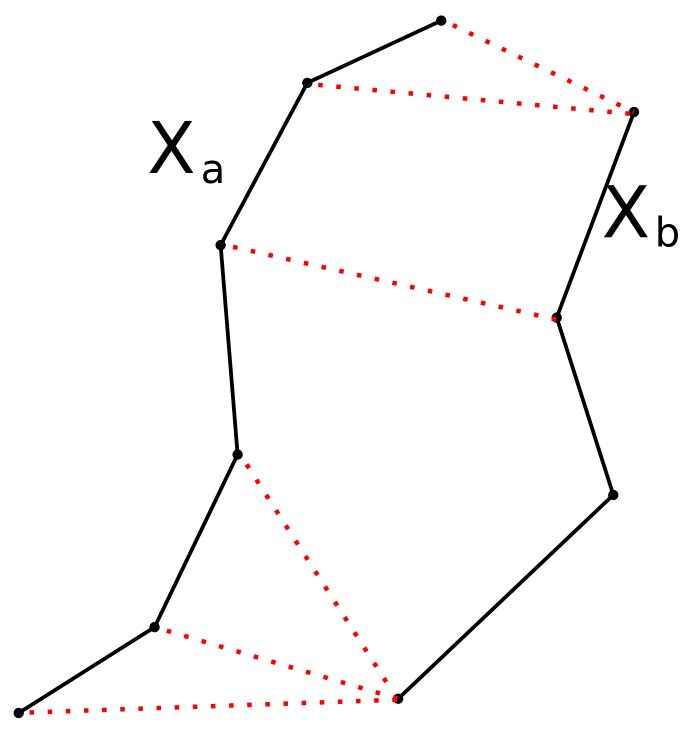
\includegraphics[width=4cm,height = 4cm]{streamline_structural_distance.pdf}
  \caption{Many distances between two streamlines, $s_A$ and $s_B$
    (solid line), that are proposed in the literature are based on the
    set of minimum distances between each point of $s_A$ to $s_B$.
    The set of minimal distances is represented here as dotted lines.}
  \label{fig:structural_distance}
\end{figure}

%\subsubsection{STAPLE sensitivity and specificity score}
%\label{subsec:experiments_quatification_staple}
%some text here

\subsubsection{Proposed method for hypotesting}
\label{subsec:experiments_quatification_proposedmethod}
From the prior knowledge of neuroscientists and doctors, there is an evidence about the reducing of the number of fibers in CST of ALS patient compared with control people. It is also the same situation with the volume of CST. Beside the number of fibers and the volume, FA and MD also play an important role for recognizing the ALS disease \cite{horsfield2002applications}. \cite{ellis1999diffusion} shows that along the corticospinal tracts, mean diffusivity was found to be significantly increased
$(p = 0.001)$ in ALS patients (limb onset: $0.771\times10^{-3} mm^2 s^{-1}$; bulbar onset: $0.778\times10^{-3} mm^2 s^{-1}$) compared with controls ($0.732\time10^{-3} mm^2 s^{-1}$). Fractional anisotropy was significantly reduced ($p = 0.007$) in bulbar onset subjects ($0.726$) compared with controls ($0.773$), but no significant difference was found between limb onset subjects ($0.761$) and controls.
Ellis et al.\cite{ellis1999diffusion} also demonstrated a positive correlation between mean diffusivity and disease duration ($r = 0.57; p = 0.009$) but no correlation with disease severity ($p > 0.29$) or upper motor neuron involvement. On the other hand, fractional anisotropy was found to correlate with measures of disease severity (assessed using the Ashworth spasticity scale and the ALS severity scale $29$).While there was no correlation between anisotropy and disease duration ($r = -0.17; p = 0.48$), significant correlations between anisotropy and the ALS severity scale ($r = -0.63; p = 0.003$) and Ashworth spasticity scale
($r = -0.56; p = 0.007$) existed.
Following are some features effectively affecting on ALS

\begin{itemize}
	\item fiber count: the number of DTI streamlines extracted for a fiber tract
	\item fiber min/max/mean length: length in $mm$ for all streamlines belonging to a fiber tract
	\item fiber volume: number of voxels occupied by all streamlines for a particular fiber tract or the geometry cylinder bounding a particular fiber tract
	\item fiber density: the ratio between fiber count and the number of voxel
	\item FA
	\item MD
	\item fragmentation: can be quantified by the ratio between the number of fibers and the volume
\end{itemize}
These features have been used as the measurement for the correctness of tractography in \cite{wang2012comprehensive}. To correct for individual differences in head size, fiber count and tract volume were normalized by intracranial volume, which was calculated from T1-weighted images using the SIENAX program in FSL \cite{smith2004techniques, smith2002accurate, smith2002automated}. 







\vspace{-2mm}
\section{Conclusion}
\label{sec:conclusion}
\vspace{-2mm}
%the contribution of the paper
In this paper, we presented a method for addressing the problem faced when attemping to interactively visualize a large dataset. The core principle behinds the framework was to choose \emph{multiple scales for representing} the data from the hierarchical clustering. Moreover, we also proposed a function to evaluate the goodness of each chosen scale based on the concept of \emph{split factor}. We instantiate this framework with an application of building the interactive visualization large dMRI data in the procedure of tractogaphy segmentation, and provide concrete result on it performance. Experiments have shown that our method provide a significant improvement for visualization the large data at different scales, which verifies the effectiveness of the interactive hierarchical visualization. Beside, we are convinced that this method can be easily integrated to any current display techniques without having to vary the data or the interactive exploration tool. 

%what is the limitation of our proposed methods and/or future works
\vspace{1mm}
As mention is the section~\ref{sec:methods}, the level of detail of each cluster, $s(C_i)$, can be computed based on radius or heigh~\cite{yang2003interactive}. In this paper we choose the multiple scales only based on the heigh of cluster. The same job but based on the radius needs to be investigated. Moreover, this work is a part of an going resarch project focusing on computer-aided tractography segmentation, where machine learning techniques are used to assist medical practitioners to do the segmentaion task more easily, flexibly  and effectively. In the future, we want to further improve the interactive segmentation tool by providing the function of adding or eleminating data points $x$ into or from the current dataset $\mathcal{X}$, and updating the visualization result without re-run the clustering algorithm.

\vspace{-3mm}



%\bibliographystyle{plainnat}
\bibliographystyle{splncs}
\bibliography{ntbaovn-cut_hierarchical_tree}

%\begin{thebibliography}
%\input{ntbaovn-cut_hierarchical_tree.bib}
%\end{thebibliography}

\end{document}
